\section{Introduction}

Given a set $S$ of classified training examples a supervised learning algorthim attempts to create a hypothesis $h$ which correctly classifiers each class.

\subsection{Support Vector Machines}
Support Vector Machines (SVM) are

For a binary classification the decision function of the SVM is the dot product of the weight vector and the training example in the feature space added to a bias vector as shown in Equation \ref{eq:BCSVM}.

\begin{equation}
\label{eq:BCSVM}
f \left ( \vec{x} \right ) = \left \langle \vec{x} \phi(\vec{x}) \right \rangle + \vec{b}
\end{equation}
where $\phi(\vec{x})$ is a mapping to the higher dimensional space.
The learning in the SVM is then finding the optimal values of the weight vector $\vec{w}$ and the basis $\vec{b}$.

The radial basis function (Equation \ref{eq:RBF}) is a common kernal function used to map the input vector $\vec{x}$ into a higher dimension.
\begin{equation}
\label{eq:RBF}
k \left ( \vec{x}_i , \vec{x}_j \right ) = exp \left ( - \frac{\left \| \vec{x}_i - \vec{x}_j \right \|}{2\sigma^2} \right ) 
\end{equation}

Something about how we are trying to elarge the margin

\subsection{Ensamble Classifers}
Given an individiual classifier $h$, an enamble of classifers can be constructed of a set of indvidual classifers, $H={h_1, h_2,\dot, h_n}$.

As long as the individual classifers have uncorrelated errors when any single classifer is incorrect the other classifiers in the ensamble might correctly classify the example.

\subsection{Boosting}
Unbalanced data sets (data sets in which a majority of the values come from one class, see Figure \ref{fig:ClassDist}) are difficult for classification schemes to learn because the minority class is not well represented and tends to be thought as noise for the classifer.
Often classifiers are trained from unblananced data sets by artifically reblaning the dataset by sampling techniques; i.e. up-sampling (sampling more from the minoarty class) and down-sampling (sampling less from the majoirty class).
Boosting is an ensamble learning method in which a set of weights is maintained over the training samples and adaptively adjusted after each training itteration according to the ones that are misclasified \cite{li_adaboost_2008}.
By maintaining a weight distribution over all of the training examples, these weights could be updated to emphasize the training examples that are misclassified incorrectly.  These incorrectly classified examples could then be learned in a refinement of the classifier or by training adding a new classifer to the ensamble with the new weights.
\begin{figure*}[ht!]
	\centering
	\begin{subfigure}[b]{0.3\textwidth}
		\centering
		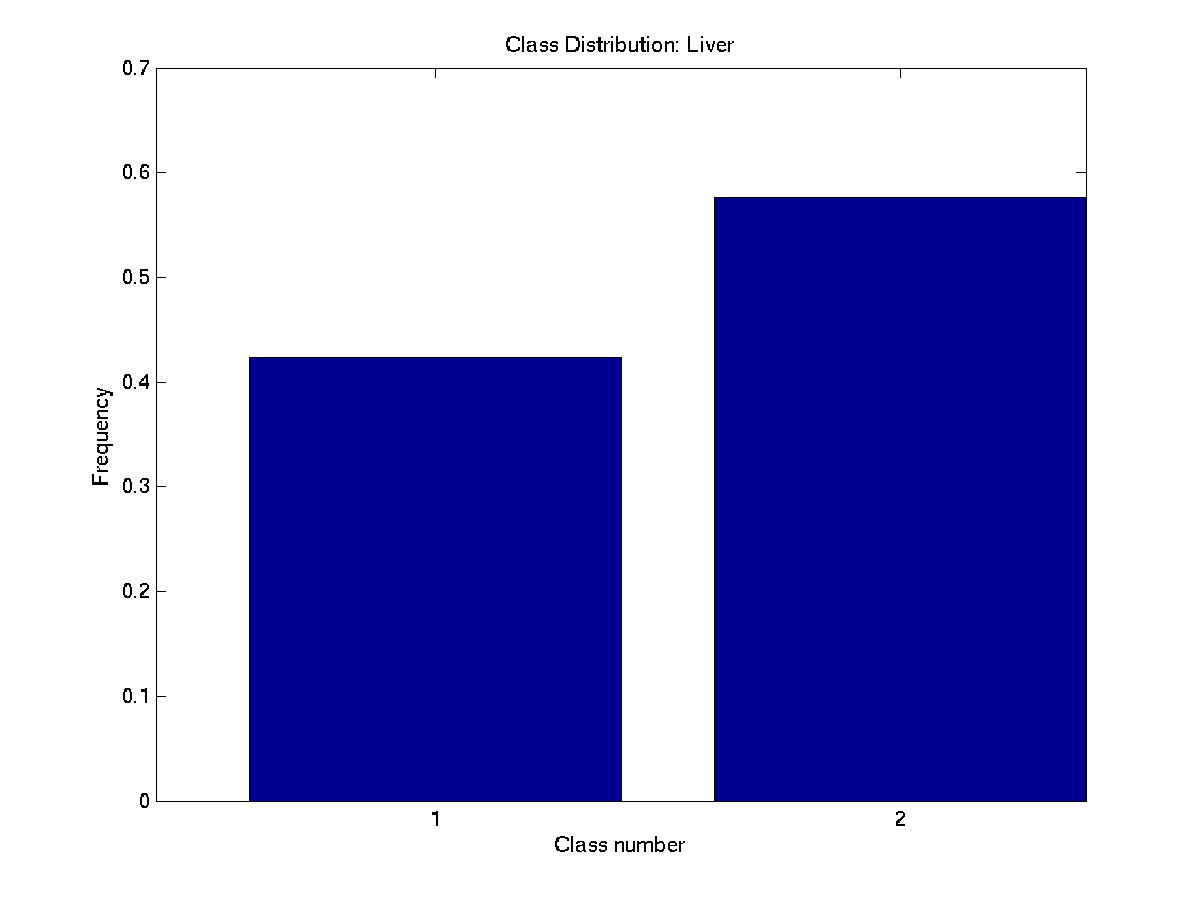
\includegraphics[width=\textwidth]{Liver_ClassDist}
        \caption{Liver}
	\end{subfigure}%
	~
	\begin{subfigure}[b]{0.3\textwidth}
		\centering
		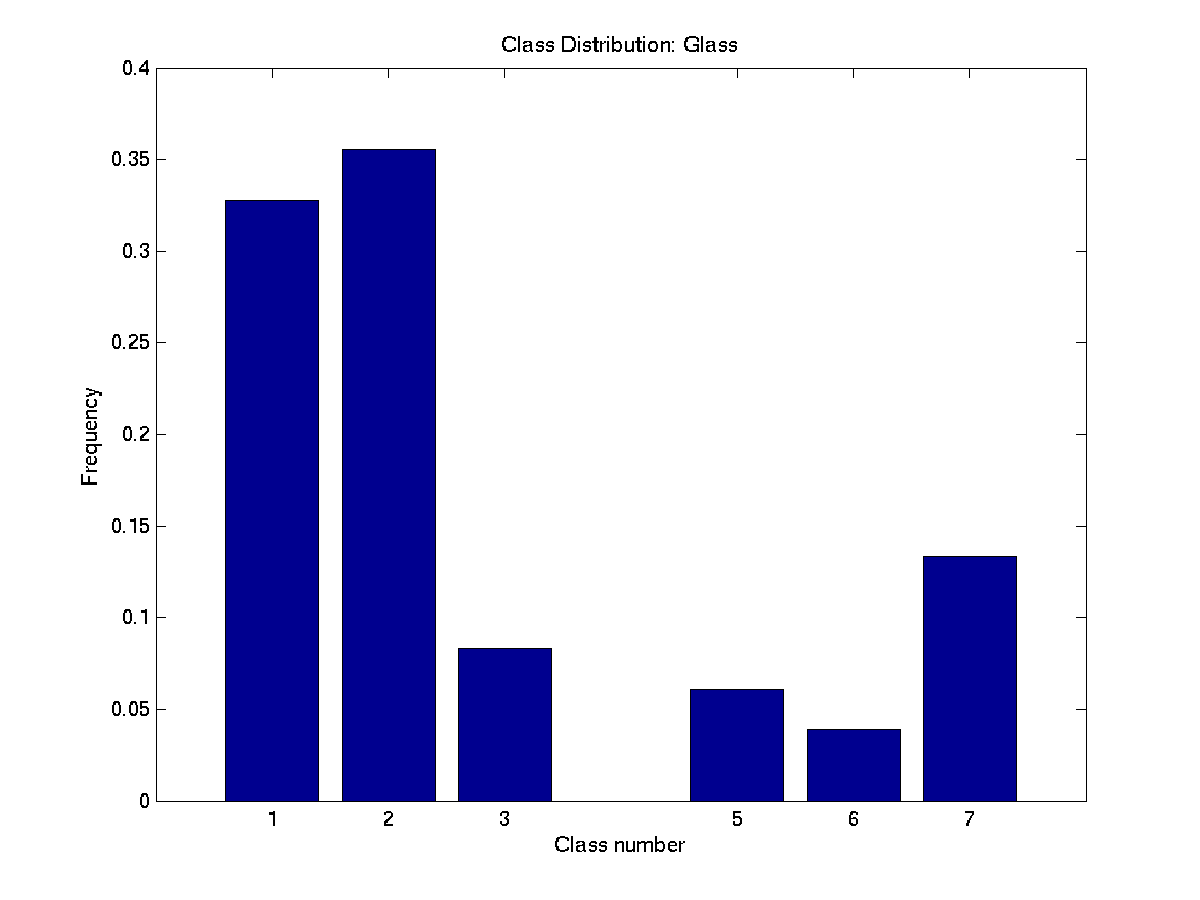
\includegraphics[width=\textwidth]{Glass_ClassDist}
        \caption{Glass}
	\end{subfigure}	
    ~
	\begin{subfigure}[b]{0.3\textwidth}
		\centering
		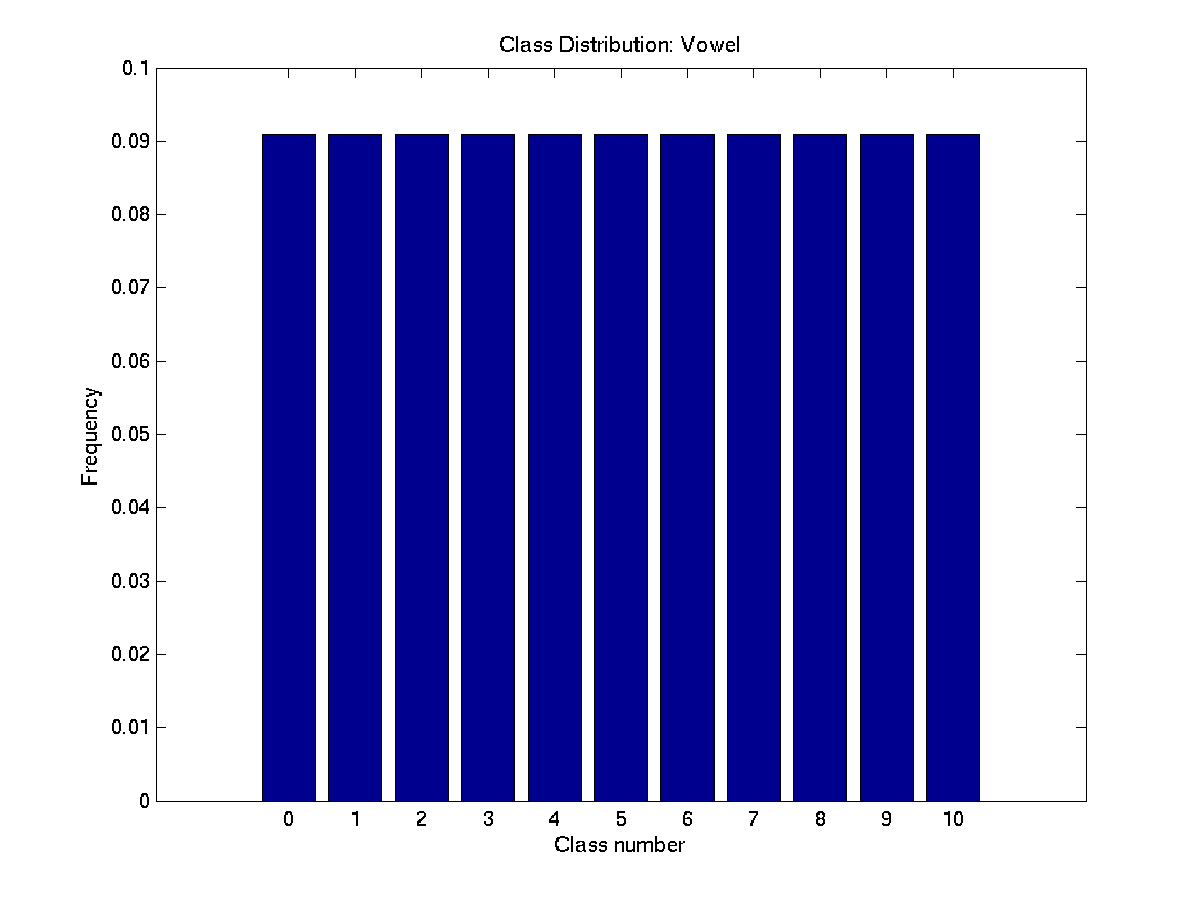
\includegraphics[width=\textwidth]{Vowel_ClassDist}
        \caption{Vowel}
	\end{subfigure}%
	\caption{Distribution of Class Data}
	\label{fig:ClassDist}
\end{figure*}
